\documentclass[a4paper]{article}%{{{

\usepackage[utf8]{inputenc}
\usepackage[T1]{fontenc}
\usepackage{textcomp}
\usepackage{url}
\usepackage{hyperref}
\usepackage[top=2.5cm,bottom=2.5cm,right=2cm,left=3cm]{geometry}
\usepackage[french]{babel}
\usepackage[backend=biber,style=ieee]{biblatex}
\usepackage{glossaries}
%\usepackage{titletoc}% http://ctan.org/pkg/titletoc
\usepackage{qtree}
\usepackage{listings}
\usepackage{xcolor}
\usepackage{setspace}
\usepackage{graphicx}
\usepackage{geometry}
\usepackage{titlesec}

% option format paragraph
\titleformat{\paragraph}
{\normalfont\normalsize\bfseries}{\theparagraph}{1em}{}
\titlespacing*{\paragraph}
{0pt}{3.25ex plus 1ex minus .2ex}{1.5ex plus .2ex}

\addbibresource{refs.bib}

\definecolor{codegreen}{rgb}{0,0.6,0}
\definecolor{codegray}{rgb}{0.5,0.5,0.5}
\definecolor{backcolour}{rgb}{0.95,0.95,0.92}
\definecolor{backpink}{rgb}{1,0.94,0.95}

\lstdefinestyle{codestyle}{
    backgroundcolor=\color{backcolour},
    commentstyle=\color{codegreen},
    keywordstyle=\color{magenta},
    numberstyle=\tiny\color{codegray},
    stringstyle=\color{teal},
    basicstyle=\ttfamily\footnotesize,
    breakatwhitespace=false,
    breaklines=true,
    captionpos=b,
    keepspaces=true,
    %numbers=left,
    %numbersep=5pt,
    showspaces=false,
    showstringspaces=false,
    showtabs=false,
    tabsize=2
}

\lstdefinestyle{grammarstyle}{
    backgroundcolor=\color{backpink},
    commentstyle=\color{codegreen},
    keywordstyle=\color{purple},
    numberstyle=\tiny\color{codegray},
    stringstyle=\color{teal},
    basicstyle=\ttfamily\footnotesize,
    breakatwhitespace=false,
    breaklines=true,
    captionpos=b,
    keepspaces=true,
    %numbers=left,
    %numbersep=5pt,
    showspaces=false,
    showstringspaces=false,
    showtabs=false,
    tabsize=2
}

\lstnewenvironment{code}[1][]
  {\noindent\minipage{\linewidth}\medskip
   \lstset{basicstyle=\ttfamily\footnotesize,frame=single,#1,upquote=true}
    \lstset{style=codestyle}
     }
  {\endminipage}

 \lstnewenvironment{grammar}[1][]
  {\noindent\minipage{\linewidth}\medskip
   \lstset{basicstyle=\ttfamily\footnotesize,frame=single,#1,upquote=true}
   \lstset{style=grammarstyle}
   }
  {\endminipage}

%===========style & geometry===========
%\lstset{style=mystyle}

 \geometry{
 a4paper,
  left=30mm,
  right=20mm,
  top=25mm,
  bottom=25mm,
 }

 \titleformat*{\subsection}{\LARGE\bfseries}
 \titleformat*{\subsubsection}{\Large\bfseries}

%================infos=================
\pagenumbering{gobble}
\begin{titlepage}

\title{Création d'un langage interprété}
\author{Franck ALONSO, CHASSAGNOL Rémi}
\date{\today}
\end{titlepage}
%}}}
%===============Glossaire==============
\makeglossaries
\newglossaryentry{ast}
{
    name=AST,
    description={(Abstract Syntax Tree) structure sous forme d'arbre utilisée
                 pour représenter une grammaire.}
}
\newglossaryentry{bnf}
{
    name=forme de Backus-Naur,
    description={métalangage utilisé pour décire les langages de programmation.}
}
\newglossaryentry{varFonc}
{
    name=fonctions variadiques,
    description={fonction qui prend un nombre indéfini de paramètres.}
}


%------------------------------------------------------------------------------%
%                                  Title page                                  %
%------------------------------------------------------------------------------%
\begin{document}
\begin{titlepage}
    
\includegraphics{img/logo_isima_inp.jpeg}
       \begin{center}
           \vspace*{1cm}
               
           \Huge
           \textbf{Création d'un langage interprété}
               
           \vspace{0.5cm}
           \LARGE
           Rapport d'élève ingénieur\\
           Projet de 2\up{ème} année\\
           Filière F2 : Génie Logiciel et Systèmes Informatiques
               
           \vspace{1.5cm}
               
           Présenté par : \textbf{Franck ALONSO} et \textbf{Rémi CHASSAGNOL}
               
           \vfill
               
           \vspace{0.5cm}
         \end{center}          
   
               
           \large
           \noindent
           Responsable ISIMA : \hfill \textbf{Mardi 31/01/2023}\\~\\
           \raggedleft \textbf{Projet de 60h}\\~\\
           \raggedright
           Campus des Cézeaux. 1 rue de la Chébarde. TSA 60125. 63178 Aubière CEDEX\\
     
               
   
   \end{titlepage}
\clearpage{}

%------------------------------------------------------------------------------%
%                                Remerciements
%------------------------------------------------------------------------------%
\subsection*{Remerciements}

\doublespacing
\large % TODO: reformuler
Nous tenons à exprimer notre profonde gratitude à :\\
- Notre encadrant et cher professeur M. Loïc YON pour al qualité de son
  encadrement, et pour nous avoir guidées durant toute la période du projet.\\
- Mme Murielle MOUZAT, notre professeur de communication pour son aide précieuse
  et indispensable pour la réussite de notre projet de 2\up{ème} année.\\

\noindent Finalement, nous exprimons nos vifs remerciements à toute personne
ayant participée de près ou de loin au bon déroulement de ce projet.

\normalsize
\onehalfspacing

\clearpage{}

%------------------------------------------------------------------------------%
%                               Table of contents
%------------------------------------------------------------------------------%
\pagenumbering{arabic}
\thispagestyle{empty}
\tableofcontents
\clearpage{}

%------------------------------------------------------------------------------%
%                               Table of figures
%------------------------------------------------------------------------------%
\listoffigures
\clearpage{}


%------------------------------------------------------------------------------%
%                              Résumé et Abstract
%------------------------------------------------------------------------------%
\setcounter{secnumdepth}{3}
\subsection*{Résumé}

Ce projet s'inscrit dans le cadre du projet commun de la filière génie logiciel
dont l'objectif est la création d'outils de démonstration servant à présenter la
filière. Notre travail a consisté en la création d'un langage de programmation
transpilé simple. Le programme doit lire un fichier de code source et de le
traduire en code python. Il doit être capable de détecter les erreurs de
syntaxes et de les spécifier à l'utilisateur. De plus, le langage est à typage
statique, de ce fait, le programme doit aussi être capable de détecter les
erreurs de types.\\

Le développement a été réalisé avec le langage C++ et emploi le paradigme objet.
De plus, nous avons utilisé les outils GNU Flex et GNU Bison pour la création du
parseur. À noter que le programme ne nécessite pas de système d'exploitation
particulier, cependant, il requière l'installation des outils cités précédemment
ainsi qu'une version de python3 pour fonctionner. % TODO: la fin ?
\\~\\

\noindent
Mots-clés : \textbf{C++}, \textbf{transpileur}, \textbf{lexeur}, \textbf{parseur},
\textbf{flex}, \textbf{bison},  \textbf{langage de programmation}
\\[2\baselineskip]

\subsection*{Abstract}

This project is a part of the common project of the software development
pathway. The objective is to create a tool for presenting software development.
Our work consisted in the creation of a simple transpiled programming language.
The program has to be able to read a source code file and generate a python
program. It must detect syntax errors in the and report theme to the user.
Furthermore, the language is statically typed so the program also has to detect
and report type errors.\\

The development has been done using C++ and object oriented programming.
Moreover, we have used the tools GNU Flex and GNU Bison to generate our parser.
We can notice that the program doesn't require any particular operating system,
however the tools previously quoted and a version of python3 have to be
installed.
\\~\\

\noindent
Keywords : \textbf{C++}, \textbf{transpiler}, \textbf{lexer}, \textbf{parser},
\textbf{flex}, \textbf{bison}, \textbf{programming language}

\clearpage{}

%------------------------------------------------------------------------------%
%                                 Introduction
%------------------------------------------------------------------------------%
\clearpage
\subsection*{Introduction}
\large
Dans le cadre du projet de 2\up{ème} année à l'ISIMA, nous avons choisi de
réaliser un travail concernant le sujet commun de la filière 2, génie logiciel
et systèmes d'informations. Le but du projet commun est la création d'outils de
démonstration servant à présenter la filière.\\

Nous souhaitions au départ, créer un langage de programmation interprété ainsi
qu'un IDE, cependant, ce projet s'est avéré trop ambitieux pour être réalisé en
60 heures. Pour simplifier, nous avons décidé de concevoir un langage transpilé,
délégant ainsi une partie des tâches complexes comme la gestion de la mémoire à
un compilateur existant.\\

Ce projet permettra de présenter un langage de programmation très simple pour
introduire des lycéen à la programmation. De plus, il pourra constituer une
maquette pour les élèves de l'ISIMA souhaitant étudier le fonctionnement des
compilateurs.\\

Pour présenter ce projet, nous commencerons par la forme du langage à créer
souhaité, puis nous détaillerons sa structure. Une fois familiarisé avec les
différentes étapes de son implémentation,  nous introduirons les concepts et
outils informatiques qui permettent la réalisation de notre langage.\\

\normalsize
\clearpage{}

%------------------------------------------------------------------------------%
%                                     Plan                                     %
%------------------------------------------------------------------------------%

% NOTE: les partie ne sont pas très équilibrées

\section{Contexte du projet}

\subsection{Création d'un langage de programmation transilé}

\subsection{Analyse du problème}

\section{Réalisation et conception}

\subsection{Conception des éléments du langage}

\subsubsection{Définition de la grammaire}

Avant d'implémenter notre langage, il faut avoir une idée de sa grammaire.
Puisque nous souhaitons utiliser ce langage à des fins pédagogiques, nous avons
décidé de simplifier au maximum la syntaxe. Par exemple, nous avons choisit de
supprimer tous les opérateurs, ainsi, toutes les opérations arithmétiques et
booléennes auront la même syntaxe que les fonctions. Par exemple, $a+b$ s'écrira
\textit{add}(\textbf{a}, \textbf{b}). De plus, pour différer au maximum de
python, notre syntaxe s'inspirera de celle des langages \textbf{C} et
\textbf{Rust}. Pour définir la grammaire de manière formelle, nous utiliserons
la \gls{bnf}.

\paragraph{Les variables}


Pour stocker des données, notre langage utilise des variables dont la
convention de nommage est la même qu'en \textbf{C}. Le langage est à typage
statique, ce qui signifie que toutes les variables doivent être déclarées avec
leur type avant d'être utilisées. Pour l'instant, nous possédons trois types :
les entiers (\textit{int}), les nombre à virgule flottante (\textit{flt}) et les
caractères (\textit{chr}). Voici la syntaxe pour déclarer une variable:

\begin{grammar}
<identifier> ::= 'a'-'z'( <alpha> | '0'-'9' )*
<int> ::= "int"
<flt> ::= "flt"
<chr> ::= "chr"
<type> ::= <int> | <flt> | <chr>
<declaration> ::= <type> <identifier> ";"
\end{grammar}\leavevmode\newline

A noter qu'ici, on a une légère différence avec le C pour le nom des fonctions
et des variable (\textbf{identifier} ici). En effet, la convention du C précise
qu'un nom de variable ou de fonction doit commencer avec une lettre minuscule,
cependant il est tout a fait possible de commencer un nom de variable par une
majuscule. Dans notre cas, les noms commencent forcément par une minuscule ce
qui force l'utilisateur à respecter notre guide de style.


\paragraph{Les fonctions}

Pour définir des fonctions, nous utilisons le mot clé \textbf{fn}, suivit du nom
de la fonction avec ses paramètres entre parenthèses et enfin le bloque de code
qui contient les instructions entre accolade. De plus, il faut spécifier le type
de la valeur retour de la fonction en utilisant \textbf{-> type} quand c'est
nécessaire.

\begin{grammar}
<function> ::= fn <identifier>"("<parameters>")" [ "->" <type> ] "{"<instructions>"}"
\end{grammar}\leavevmode\newline

Pour pouvoir retourner une valeur, il faudra utiliser le mot clé \textit{return}
dans la fonction.

\paragraph{Les structures de contrôle}

Nous avons aussi ajouté les structures de contrôle présentes dans la plupart des
langages de programmation.

\begin{grammar}
<if> ::= if "("<condition>")" "{"<instructions>"}" [ else "{" <instructions>"}" ]

<range> ::= range "("<valueSymbol>, <valueSymbol>, <valueSymbol>")"
<for> ::= for <identifier> in <range> "{"<instructions>"}"

<while> ::= while "("<condition>")" "{" <instructions> "}"
\end{grammar}\leavevmode\newline

\paragraph{Les opérations}

Comme dit précédemment, tous le langage ne comporte pas d'opérateur donc toutes
les opérations se font à l'aide de fonctions directement intégrées dans le
transpileur. Voici une liste des opérations possibles :

\begin{center}
\begin{tabular}{ | c | c | }
    \hline
    opération & syntaxe\\
    \hline
    \textbf{a} + \textbf{b} & \textit{add}(\textbf{a}, \textbf{b})\\
    \hline
    \textbf{a} - \textbf{b} & \textit{mns}(\textbf{a}, \textbf{b})\\
    \hline
    \textbf{a} $\times$ \textbf{b} & \textit{tms}(\textbf{a}, \textbf{b})\\
    \hline
    \textbf{a} $\div$ \textbf{b} & \textit{div}(\textbf{a}, \textbf{b})\\
    \hline
    \textbf{a} \textbf{==} \textbf{b} & \textit{eql}(\textbf{a}, \textbf{b})\\
    \hline
    \textbf{a} \textbf{<} \textbf{b} & \textit{inf}(\textbf{a}, \textbf{b})\\
    \hline
    \textbf{a} \textbf{>} \textbf{b} & \textit{sup}(\textbf{a}, \textbf{b})\\
    \hline
    \textbf{a} \textbf{<=} \textbf{b} & \textit{ieq}(\textbf{a}, \textbf{b})\\
    \hline
    \textbf{a} \textbf{>=} \textbf{b} & \textit{seq}(\textbf{a}, \textbf{b})\\
    \hline
    \textbf{not} \textbf{a} & \textit{not}(\textbf{a})\\
    \hline
\end{tabular}
\end{center}

\paragraph{Entrée et sortie}

Le langage possède aussi la possibilité d'afficher et de lire du texte depuis la
console. La lecture se fait avec la fonction \textit{read} qui prend en
paramètre une variable qui stockera le résultat. Pour la l'affichage, il faudra
utiliser la fonction \textit{print} qui peut être utilisée de deux manières :

\begin{itemize}
  \item \lstinline{print("Hello, World!")} : affiche du texte
  \item \lstinline{print(variable)} : affichage d'une valeur.
\end{itemize}

Nous n'avons pas implémenter de fonction d'affichage similaire à \textbf{printf}
en C. La première raison est le fait que notre langage ne supporte pas les
\gls{varFonc}. De plus, l'ajout de ce type de fonctions d'affichage nécessite la
gestion d'une chaine de formatage, ce qui aurai grandement augmenté la
complexité de notre grammaire si nous avion voulu l'intégrer directement au
langage.

\paragraph{Exemple de code}

Dans cet exemple, nous disposons de 2 variables \textbf{a} et \textbf{b}. La
variable \textbf{a} est lue par commande de l'utilisateur tandis que la valeur 4
est assignée à \textbf{b}.\\
Nous cherchons ensuite à additionner les 2 variables avec la valeur 5. Nous avons alors la syntaxe suivante :\\
- une fonction \textit{add3} qui additionne les valeurs de ses 3 paramètres\\
- une fonction \textit{affiche} qui affiche sur l'écran le nombre passé en paramètre\\
- une fonction \textit{main}, où se trouve toutes les commandes voulues de notre programme\\

% subsection  (end)


\begin{grammar}[language=C++]
fn add3(int a, int b, int c) -> int {
    return add(a, add(b, c));
}

fn affiche(int n) {
    print("nombre : ");
    print(n);
}

fn main() {
    int a;
    int b;
    read(a);
    set(b, 4);
    affiche(add3(a, b, 5));
}
\end{grammar}\leavevmode\newline

% TODO: synthèse et transition


\clearpage{}

\subsubsection{Arbre syntaxique}

Pour donner un sens aux éléments textuels du langage, nous utiliserons une
représentation sous forme d'arbre. On appel cela un arbre syntaxique ou
\gls{ast}. Les arbres syntaxiques sont nés avec la
théorie des langages et comme on peut le voir dans cet article
\cite{compilerTICH}, les \gls{ast} sont très utilisés par les compilateurs car ce sont
des structures plus simples à manipuler que du texte. Voici l'arbre syntaxique
de la fonction \textit{add3} :

\begin{figure}[h]
  \begin{center}
  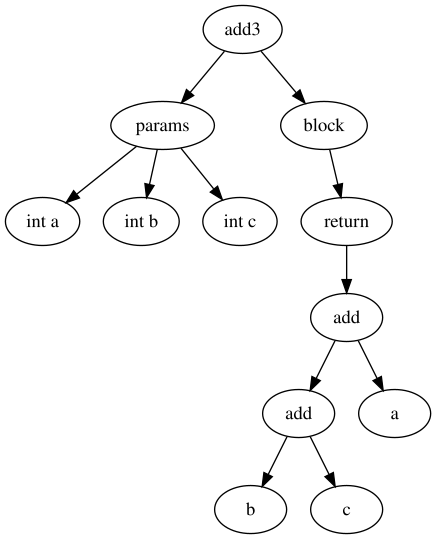
\includegraphics[scale=0.4]{img/ast1.png}
  \caption{Exemple d'arbre syntaxique}
  \end{center}
\end{figure}

Pour cette partie, nous nous sommes inspiré d'un projet appelé \textbf{minijava}
\cite{minijava} ainsi que d'un article \cite{gagnon1998sablecc} qui couvre aussi
l'utilisation des \gls{ast} en java. Nous avons choisit l'approche objet, avec un AST
représenté par des classes, où chaque nœud de l'arbre a sa propre classe.\\

Toutes les classes de l'arbre sont stockées dans le fichier
\lstinline{AST/AST.hpp} et héritent toutes d'une classe abstraite
\lstinline{ASTNode}. L'emploi de l'héritage ici est très important car
nous profiterons par la suite des avantages du polymorphisme pour stocker des
opérations de différents types. La classe \lstinline{ASTNode} est abstraite car
elle ne doit pas être instanciée, il faut que chaque nœud ai un type concret
utilisable dans le transpileur. Le diagramme de classes complet est disponible
en annexe \ref{appendix:classAST}. Détaillons maintenant les parties
importantes.

\paragraph{Les bloques de code}

La classe \lstinline{Block} correspond aux bloques de code en entre accolades.
Elle possède une liste de nœuds qui sont les opérations contenues dans le
bloque.

\clearpage{}
\paragraph{Les conteneurs d'opérations}

La classes \lstinline{Statement} correspond aux éléments qui contiennent des
blocks de code. Cela comprend les fonctions et les structures de contrôles. La
grammaire ne permet pas l'emploi des bloques ailleurs.

\begin{figure}[h!]
  \begin{center}
  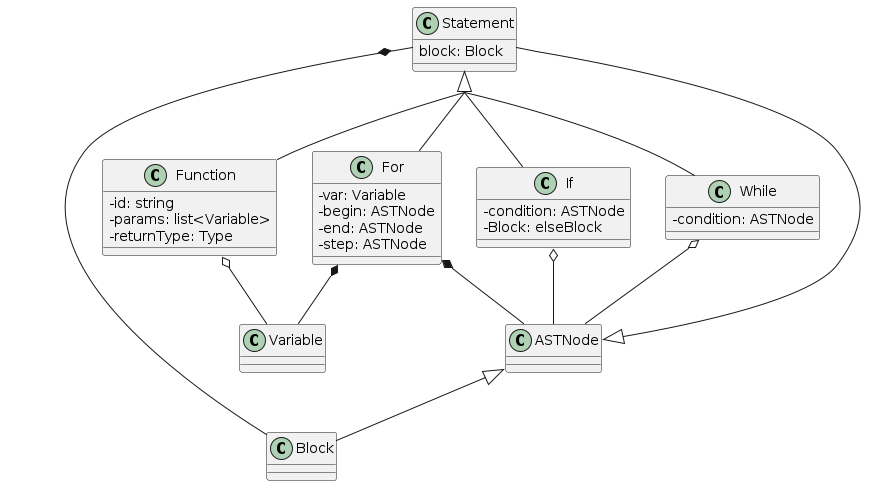
\includegraphics[scale=0.5]{../ressources/diagrams/stmts.png}
  \caption{Diagramme de classe: Statement}
  \end{center}
\end{figure}

\paragraph{Les opérations}

Les opérations sont traitées avec la classe \lstinline{OperationBinaire} qui
correspond à tous les opérateurs.

\begin{figure}[h!]
  \begin{center}
  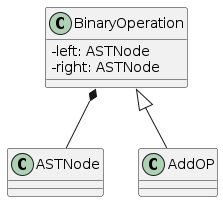
\includegraphics[scale=0.5]{../ressources/diagrams/binaryOp.png}
  \caption{Diagamme de classe: BinaryOperation}
  \end{center}
\end{figure}

\clearpage{}
\paragraph{Les éléments typé}
\label{sec:eltTypes}

Les fonctions, les valeurs et les variables possède un champ type. \textbf{Type}
est une énumération qui possède les éléments suivant :

\begin{figure}[h!]
  \begin{center}
  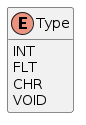
\includegraphics[scale=0.5]{../ressources/diagrams/Type.png}
  \caption{Enumération Type}
  \end{center}
\end{figure}

Les valeurs et les variable possède un simple type, et les fonctions possède une
liste de \textbf{Type} qui contient le type des paramètres suivit du type de
retour de la fonction. À noter que pour stocker une valeur, on utilise une union
composé d'un entier, d'un double et d'un char. De ce fait, \textbf{Value} peut
contenir n'importe quel type de valeur et le champ à utiliser est déterminé par
le type de la valeur.


\clearpage{}

\subsection{Construction de l'AST}

Dans cette partie nous expliquerons la création d'un parseur en utilisant les
outils \textbf{GNU Flex} et \textbf{GNU Bison}. De plus, nous détaillerons la
génération de l'AST en utilisant les classes décrites précédemment. Pour cette
partie, nous nous sommes aidé d'un article \cite{compilerFlexBison} qui présente
la construction d'un compilateur avec Flex et Bison en C. Pour porter le code en
C++, nous avons utilisé la documentation officielle des deux outils ainsi qu'un
article qui nous a permis d'avoir un squelette de base pour le lexeur et le
parseur \cite{cppparsing}.

\subsubsection{Le lexeur}

\phantomsection
\paragraph{Définition}

Le lexeur, ou encore appelé analyseur lexical, a pour but de transformer le
texte du code source en des unités lexicales, appelées \textit{tokens}
\cite{flexBisonHandbook}. \\

\paragraph{Exemple}

Pour l'expression simple \textbf{a = 2 * b} \\
Les tokens apparaissant sont : \\
\begin{center}
  \begin{tabular}{ | c | c | }
    \hline
    \textbf{Token} & \textbf{Sa nature} \\
    \hline
    a & Identificateur de variable \\
    \hline
    = & Symbole d'affectation \\
    \hline
    2 & Valeur entière \\
    \hline
    * & Opérateur de multiplication \\
    \hline
    b & Identificateur de variable \\
    \hline
  \end{tabular}
\end{center}

Le lexeur a également pour rôle de supprimer les informations inutiles,
généralement du caractère blancs (espaces et tabulations) et des
commentaires.\\~\\

\phantomsection
\paragraph{Implémentation}

L'outil utilisé pour générer le lexeur est \textbf{GNU Flex} (Fast LEXical
analyser generator). Il permet de générer le code C++ du lexeur à partir d'un
fichier. Dans notre cas, le fichier utilisé sera \textbf{main\_cpp.l} et possède
la structure suivante \cite{compilerFlexBison} :

\begin{code}
// code C++, options et declarations de raccourcis

%%
// Definition des tokens et actions

%%
// Fonctions C++
\end{code}\leavevmode\newline

\noindent

Dans la première partie en haut du fichier, on place les inclusions de
bibliothèques C/C++ ainsi que des options pour flex.

\begin{code}
%{
#include "parser.hpp"
#include "lexer.hpp"
%}

%option c++ interactive noyywrap yylineno nodefault outfile="lexer.cpp"
\end{code}\leavevmode\newline

Détail des fonctions utilisée :
\begin{itemize}
  \item \textbf{c++} : indique qu'on travail avec du cpp et non du c
  \item \textbf{interactive} : utile quand on utlise \textbf{std::in}. Le
    scanner interactif regarde plus de caractères avant de générer un token
    (plus lent mais permet de lutter contre les ambiguitées)
  \item \textbf{noyywrap} : ne pas appeler \textbf{yywrap()} qui permet de parser plusieurs fichiers
  \item \textbf{nodefault} : pas de scanner par défaut (=> on doit tout implémenter)
  \item \textbf{outfile:"file.cpp"} : permet de definir le fichier de sortie
\end{itemize}\leavevmode\\

% TODO: dvlp sur les règles
Après les options on peut définir des raccourcis en utilisant des expressions
régulières. Par exemple, dans le code ci-dessous, nous avons définit les règles
suivantes :

\begin{itemize}
  \item \textbf{alpha :} un caractère alphabétique est composé d'une lettre
    minuscule ou d'une lettre majuscule.
  \item \textbf{digit :} les chiffres sont les caractères entre 0 et 9.
  \item \textbf{int :} les entiers correspondes à une suite de chiffres et
    peuvent être positifs ou négatifs.
  \item \textbf{float :} similaire aux entiers sauf qu'ici on a obligatoirement
    un point suivit d'une suite de chiffre à la fin.
  \item \textbf{char :} les caractère sont toujours écrit entre \textbf{'} (par
    exemple \textbf{'a'}).
  \item \textbf{identifier :} correspond aux noms de fonctions et de variables
    et suit le standard du C. Un identifiant commence par une lettre minuscule
    et peut être suivit d'une suite de lettres, de nombre et de \textbf{\_}.
\end{itemize}

\begin{code}
alpha [a-zA-Z]
digit [0-9]
int [+-]?{digit}+
float [+-]?{digit}+\.{digit}+
char '{alpha}'
identifier [a-z]({alpha}|{digit}|_)*
\end{code}\leavevmode\newline

\noindent

Dans la seconde partie du fichier, on définit des règles et des actions. À noter
que l'on peut utiliser les raccourcis définis précédemment en mettant leurs noms
entre accolades comme fait ci-dessous pour \textbf{identifier}. La définition
d'une règle suit le principe suivant, on commence par donner une suite de
caractères qui sera consommée. Ensuite met du code entre accolades, et ce code
sera exécuté quand le lexeur consommera la chaine. Par exemple, si on prend la
première ligne ci-dessous, quand le lexeur trouvera le mot \textbf{for}, il
affichera \textit{L\_for} dans le terminal puis retournera le token \textbf{FOR}.

À noter que les tokens disponibles dans l'espace de nom \textbf{Parser::token}
doivent être définis dans le ficher bison que l'on détaillera dans la partie
suivante.

\begin{code}
for          { AFFICHE("L_for"); return Parser::token::FOR; }
{identifier} {
  AFFICHE("L_id");
  yylval->build<std::string>(yytext);
  return Parser::token::IDENTIFIER;
}
\end{code}\leavevmode\newline

\noindent

Ici on a accès à la variable \textcolor{purple}{yylval} de type
\textcolor{purple}{Parser::semantic\_type*} qui possède une méthode
\textcolor{purple}{build} permettant de transmettre des valeurs à bison.\\

% TODO: ça doit pas être là je pense
% Ces valeurs sont accessibles via les variables de bison: \textcolor{purple}{\$2}. La variable
% \textcolor{purple}{yytext} contient le text traité par Flex. De plus, dans le code, on retourne
% les \textit{tokens}. Ces \textbf{tokens} sont définis dans le fichier de bison.
% \newline

La fonction appelée par défaut est \textcolor{purple}{yylex}, cependant, pour
pouvoir travailler avec bison, nous devons fournir nos propres fonctions, pour
ce faire on utilise la macro \textcolor{purple}{YY\_DECL}, comme expliqué dans
la partie \textit{9 The Generated Scanner} du manuel pour Flex
\cite{flexmanual}.

\begin{code}
#define YY_DECL int interpreter::Scanner::lex(Parser::semantic_type *yylval, Parser::location_type *yylloc)
\end{code}\leavevmode\\~\\

Cette macro permet de définir le type de la fonction \textbf{lex}, ici,
on a pour paramètre \textcolor{purple}{yylval} (qui comme dit précédemment permet
de transmettre des valeurs à bison) et \textcolor{purple}{yylloc} qui doit être
fourni quand on utiliser les positions dans le parseur (pour avoir le numéro de
ligne en cas d'erreur par exemple), mais cela nécessite une option particulière
pour bison.

\clearpage{}

\subsubsection{Le parseur}

\phantomsection
\paragraph{Définition}

Également appelé analyseur syntaxique, son rôle principal est la vérification de
la syntaxe du code en regroupant les tokens selon une structure suivant des
règles syntaxiques. \\


\paragraph{Exemple}

Pour l'expression simple \textbf{a = 2 * b} \\
Les tokens apparaissant sont : \\
\begin{center}
\begin{tabular}{ | c | c | c | }
\hline
\textbf{Arbre syntaxique} & \textbf{Évaluation de 2 * b} & \textbf{Affectation de a} \\
\hline
\Tree[.= a  [.* 2 b ]] &
    \Tree[.= a  2*b ] &
        a = 2 * b\\
\hline
\end{tabular}
\end{center}

\phantomsection
\paragraph{Implémentation}

À l'instar de Flex pour le lexeur, Bison est un générateur de grammaire qui
convertit une description de grammaire en un programme C++ qui analyse cette
même grammaire.\\

L'article \cite{compilerFlexBison} s'est encore une fois révélé très utile pour
la réalisation du fichier nécessaire à Bison\\~\\

Le fichier \textbf{main\_cpp.y} contient le code qui permet de générer le
parseur avec Bison. Toutes les règles syntaxiques qui définissent la grammaire
du langage y sont comprises. Chaque règle va contenir des bloques de code qui
seront exécutés au moment où le parseur la reconnait, ce code permet de
construire l'ABS (Abstract Syntaxic Tree) du programme ainsi que de faire de la
vérification sur les symboles (définition et type).\\

La structure du fichier \textbf{main\_cpp.y} est similaire à celle du lexeur :

\begin{code}
// C++, options, et declaration des tokens

%%
// Regles de grammaire

%%
// fonctions C++
\end{code}\leavevmode\newline

Les tokens sont définis en début de fichier avec la syntaxe suivante:

\begin{code}
%token IF ELSE FOR WHILE FN INCLUDE IN
%token <long long>  INT
%token <double>     FLOAT
%token <char>       CHAR
%token <std::string> IDENTIFIER
\end{code}\leavevmode\newline

À noter que l'on peut spécifier le type de l'élément, ce qui sera utile pour
récupérer les valeurs retournées par le lexeur.\\~\\


Bison permet de construire le parser, qui va reconnaître des éléments de syntaxe
et non pas juste des mots clés. Par exemple, on peut définir une règle pour
reconnaître une suite d'inclusion de fichiers :\\

\begin{code}[language=c++]
includes: %empty
       | INCLUDE IDENTIFIER SEMI includes
       ;
\end{code}\leavevmode\newline

Ici, on définie une règle \textbf{includes} qui décrit la syntaxe des
\textit{includes}. Selon cette règle, une suite d'inclusions est soit vide, soit
elle comporte une inclusion, suivit d'une suite d'inclusion (`|` signifie "ou").
Il faut noter que la syntaxe est "récursive", ce qui nous permet de définir une
suite d'éléments. Enfin, les mots en majuscule sont les tokens retournés par le
lexeur.\\

On peut ajouter des blocks de codes qui seront exécutés au moment où le parseur
atteint l'élément qui précède le block. Dans l'exemple ci-dessous, le block sera
appelé une fois que Bison aura parser le \textcolor{purple}{;}. À noter que l'on
peut accéder aux éléments retournés par Flex ; ici, \textcolor{purple}{\$2} fait
référence au second élément de la règle qui est \textcolor{purple}{IDENTIFIER}.
Le type de \textcolor{purple}{IDENTIFIER} a été défini comme étant une
\textcolor{purple}{std::string}. Le block de code nous permet donc de créer une
nouvelle inclusion et de récupérer le nom de la bibliothèque.\\

\begin{code}[language=c++]
includes: %empty
       |
       INCLUDE IDENTIFIER SEMI
       {
         std::cout << "new include id: " << $2 << std::endl;
         pb.addInclude(std::make_shared<Include>($2));
       }
       includes
       ;
\end{code}\leavevmode\newline


Comme dit plus haut, on peut définir des types pour les tokens, ce qui permet de
récupérer des valeurs:

\begin{code}[language=c++]
value: INT {
       std::cout << "new int: " << $1 << std::endl;
       lastValue.i = $1;
       lastValueType = INT;
     } | FLOAT {
       std::cout << "new double: " << $1 << std::endl;
       lastValue.f = $1;
       lastValueType = FLT;
     } | CHAR {
       std::cout << "new char: " << $1 << std::endl;
       lastValue.c = $1;
       lastValueType = CHR;
     }
     ;
\end{code}\leavevmode\newline

Pour la génération du code, on a deux options :
\begin{itemize}
\item utiliser des instruction très simples => sorte de bytecode
\item créer un code objet où tous les éléments sont des objets.
\end{itemize}\leavevmode\\~\\

\underline{Choix de la représentation objet} :
\begin{itemize}
\item plus simple à comprendre et à visualiser
\item plus compliqué à générer: on peut générer du bytecode au fil de l'exécution du parseur, en utilisant des \textcolor{orange}{goto} pour sauter de block d'instruction en block d'instruction. Pour le code objet, les éléments à l'intérieurs des blocks doivent être créés avant le block, et le block est détecté avant les instructions, il faut donc stocker les instructions.
\end{itemize}


\clearpage{}

\subsubsection{Fabrique à programme}

Pour construire l'arbre syntaxique dans le programme, nous utiliserons
la classe \textbf{ProgramBuilder}. Cette classe permet de stocker des éléments
comme le nom de la fonction courante ou les commendes récupérée par le parseur.
De plus cette classe permet d'instancier les éléments de l'AST pour construire
le programme. Le diagramme de cette classe est le suivant :

\begin{figure}[h]
  \begin{center}
  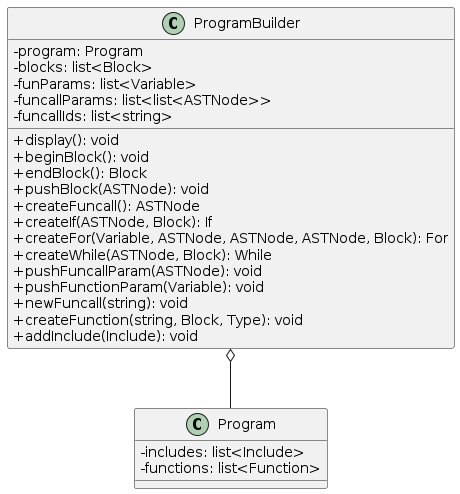
\includegraphics[scale=0.5]{../ressources/diagrams/program-builder.png}
  \caption{Diagramme de classe : ProgramBuilder}
  \end{center}
\end{figure}

On peut noter sur ce diagramme que l'on a des fonctions de créations qui
permettent de créer les éléments de l'AST définis dans la première partie. De
plus la classe est composé du programme, auquel elle ajoute les fonctions et les
fichiers inclus. % note: ça va changer

L'emploi de cette classe permet de limiter le code dans le parseur mais aussi de
pouvoir récupérer des éléments dans des piles quand on ne connait pas leurs
nombre. Par exemple, pour les \textbf{Block}, on ne sait pas combien de
commandes ils contiennent, c'est pourquoi le \textbf{ProgramBuilder} possède une
pile qui permet d'ajouter les commandes au bloques ainsi que d'avoir accès au
dernier bloque pour construire les \textbf{Statement}. Il en est de même pour
les paramètres de fonctions, dans ce cas nous avons une liste de liste. Si une
fonction \textbf{A} prend le résultat d'une autre fonction \textbf{B} en
paramètre (\textit{A(..., B(...), ...)}), la dernière liste contient les
paramètres de \textbf{B} au moment ou \textbf{B} est traitée. À l'origine, ce
choix avait été fait car il permet de toujours avoir accès aux éléments qui sont
en train d'être récupérer depuis n'importe quel endroit du parseur. Cependant,
cette fonctionnalité n'est pas utilisée, il aurait donc été plus simple de
construire ces listes en utilisant les valeurs retour de bison.\\
% NOTE: je sais plus parler

Le \textbf{ProgramBuilder} permet donc de stocker les éléments important ainsi
que de construire le \textbf{Program} au fur et à mesure de l'exécution du
parseur.


\subsection{Analyse des symboles}

Dans cette partie, nous allons créer une table des symboles qui, de façon
similaire à ce que l'on voit dans \cite{compilerFlexBison}, permet de vérifier
si les symboles (variables et fonctions) utilisés ont bien été déclarés.
Cependant, ici notre table des symboles sera plus complexe du fait que les
symboles peuvent avoir des portées différentes. De plus la table des symboles
nous permettra aussi de faire de la vérification de types pour par exemple,
vérifier qu'une fonctions prend les bon paramètres.

Du fait que nous allons devoir faire de la détection d'erreurs, nous créerons
une nouvelle classe qui permettra de stocker tous les messages d'erreurs (et
avertissements) au fil de l'exécution du parseur. Ces messages seront affichés à
la fin une fois le tous code source traité. À noter que la présence d'erreurs
empêche la compilation.

\subsubsection{Gestion des symboles}

\paragraph{La table des symboles}

Pour la création de notre table des symboles nous utiliserons la méthode
présenté dans cet article \cite{power2000symbol} que nous avons simplifié pour
la récupération et la recherche de symboles.\\

Commençons par étudier la composition d'un symbole. Chaque symbole est composé
d'un nom qui lui sert d'identifiant, d'un type et d'un genre. Le genre est une
énumération qui suis le même principe que dans \cite{power2000symbol}. Le type
du symbole est une liste de \textbf{Type} qui est une énumération décrite dans
l'AST, il a la même utilité que pour les éléments typées \ref{sec:eltTypes}.

\begin{figure}[h!]
  \begin{center}
  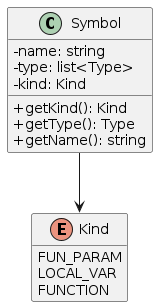
\includegraphics[scale=0.5]{../ressources/diagrams/symbol.png}
  \caption{Diagramme de classe : Symbol}
  \end{center}
\end{figure}

Pour implémenter la table des symbole nous nous sommes inspiré du schéma suivant
\cite{symtableGenius}. Ici la table des symboles est une table de tables, et
chaque sous table correspond à une zone de code dans laquelle peuvent être
définis des symboles (\textbf{scope}). Cette représentation est intéressante car
elle permet de pouvoir aisément vérifier si un symbole existe en remontant
l'arborescence de la table jusqu'aux \textbf{scope} global. En effet, les
éléments stockés dans la table mère sont toujours accessibles.
\clearpage

\begin{figure}[h!]
  \begin{center}
  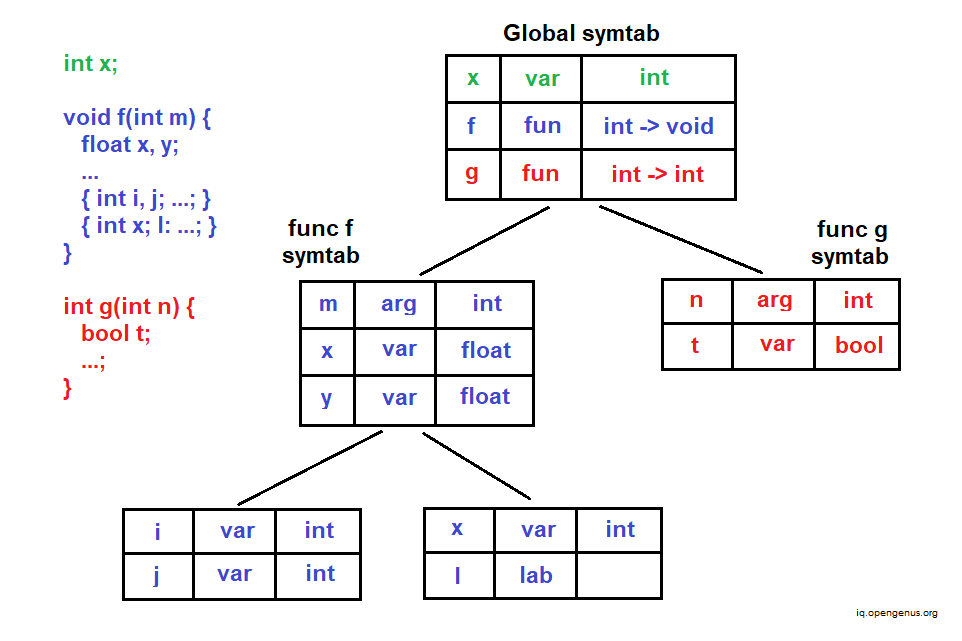
\includegraphics[scale=0.5]{./img/symtable.png}
  \caption{Structure de la table des symboles}
  \end{center}
\end{figure}

% TODO diagramme de classe

Pour l'implémentation, nous suivrons le diagramme ci-dessous. Les symboles sont
stockés dans une \textbf{unordered\_map} qui est une table de hachage qui
permettra de récupérer les symboles avec leurs identifiants. De plus, la table
possède un liste de sous tables qui et un pointeur sur la table mère qui sera
utilisé par la méthode \textbf{lookup} pour la recherche de symbole comme
expliqué précédemment.

\begin{figure}[h!]
  \begin{center}
  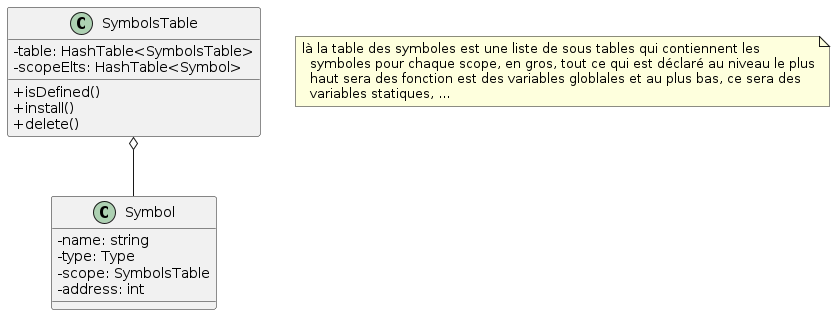
\includegraphics[scale=0.5]{../ressources/diagrams/symtable2.png}
  \caption{Diagramme de classe : Symtable}
  \end{center}
\end{figure}

\paragraph{Gestion du contexte}

% TODO: context manager

\subsubsection{Gestion des erreurs}

% TODO: errorMgr

\subsubsection{Traitement des des symboles dans le parseur}

\paragraph{Vérification des définitions}

% définition des variables
% définition des fonction

\paragraph{Vérification des types}
% fonction
% set
% vérifcation du return

\subsection{Le transpileur}
% TODO

%------------------------------------------------------------------------------%
%                                 bibliography                                 %
%------------------------------------------------------------------------------%
\clearpage{}
\printbibliography[keyword={paper},title={Biliographie}]
\printbibliography[keyword={web},title={Webographie}]

%------------------------------------------------------------------------------%
%                             Affiche le glossaire                             %
%------------------------------------------------------------------------------%
\clearpage
\printglossaries

\appendix

\clearpage{}
\subsection{Diagramme de classes de l'AST}\label{appendix:classAST}

\begin{figure}[h]
  \begin{center}
  \rotatebox[origin=c]{90}{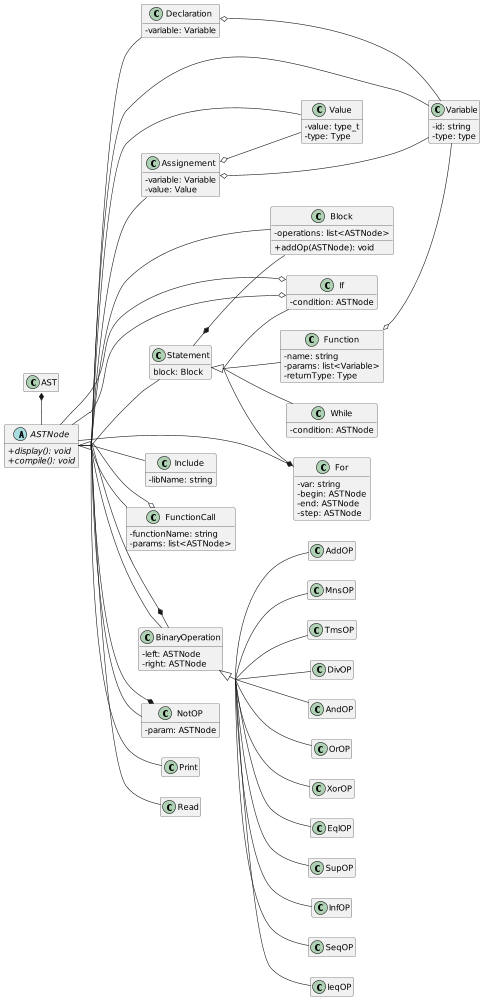
\includegraphics[scale=0.22]{../ressources/diagrams/ast.png}}
  \end{center}
\end{figure}

\end{document}


%------------------------------------------------------------------------------%
%               Résumé des réfs (à supprimer à la dernière version
%------------------------------------------------------------------------------%
% \subsection{Résumé des références}{{{
%
% \begin{itemize}
%   \item La partie consultable de \cite{flexBisonHandbook} présentent les bases
%     de flex.
%   \item \cite{compilerFlexBison} présente la construction d'un compilateur avec
%     flex et bison. Le compilateur présenté utilise une \textbf{table des
%     symboles} ainsi qu'une sorte de \textbf{byte code}. Nous avons choisi
%     l'autre méthode qui consiste à utiliser un object-ABS plutot que directement
%     du byte code. Article très utilisé au départ pour la mise en place du
%     parseur/lexeur.
%   \item \cite{flexmanual}: manuel d'utilisation de Flex.
%   \item \cite{cppparsing}: nous a permis d'avoir un exemple de code qui allie
%     flex et bison en C++ et non en C.
%
%
%   \item \cite{compilerTICH} explication du fonctionnement d'un compilateur.
%   \item \cite{compilerTILB} première version de l'article précédent.
%   \item \cite{crew1997astlog} création d'un analyser syntaxique pour du C/C++:
%     ASTROLOG. L'article par d'analyse syntaxique et de la construction
%     d'\textbf{ABS}.
%
%   \item \cite{visser2002meta} L'objectif de l'article est de présenter
%     l'utilisation des \textbf{ABS} pour de la méta programmation. Il comporte
%     pas mal d'exemples sur les \textbf{ABS} donc je le trouve pertinant.
%   \item \cite{gagnon1998sablecc}: \textbf{ABS} en java.
% \end{itemize}
%
%
% \clearpage{}
% \setcounter{secnumdepth}{1}}}}
